\documentclass[aspectratio=169,12pt]{beamer}
\usepackage{amsmath}
\usepackage{amssymb}
\usepackage{xcolor}
\usepackage[most]{tcolorbox}
\usepackage{graphicx}
\usepackage[sfdefault,lf]{FiraSans}
\renewcommand{\familydefault}{\sfdefault}
\setlength{\parindent}{0pt}
\everymath{\displaystyle}

\setbeamertemplate{navigation symbols}{}
\setbeamertemplate{footline}{}
\setbeamertemplate{headline}{}

\definecolor{mmpageWhite}{HTML}{FCFBF7}
\definecolor{mmtanSoft}{HTML}{F7F5EF}
\definecolor{mmgreenDeep}{HTML}{244B2C}
\definecolor{mmgreenLeaf}{HTML}{5D8A56}
\definecolor{mmtext}{HTML}{163221}
\definecolor{mmanswerColor}{HTML}{306A3A}

\setbeamercolor{background canvas}{bg=mmpageWhite}
\setbeamercolor{normal text}{fg=mmtext,bg=mmpageWhite}

\newtcolorbox{MMProblemCard}[1][]{enhanced,breakable=false,colback=white,colframe=black,boxrule=1.0pt,arc=5pt,left=3pt,right=3pt,top=2pt,bottom=2pt,before skip=0pt,after skip=0pt,height=0.22\textheight,valign=top,#1}
\newcommand{\KoruIcon}{\raisebox{-0.2em}{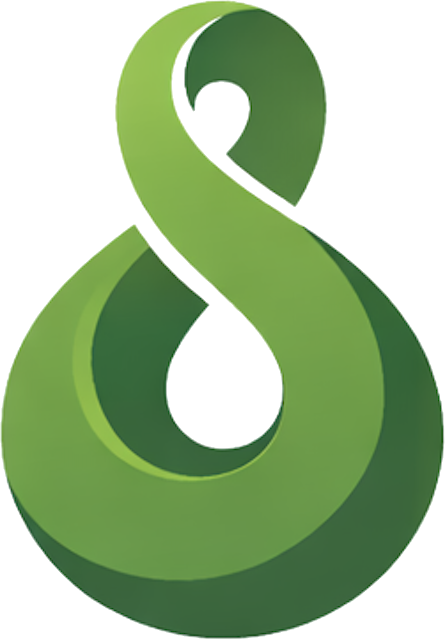
\includegraphics[height=1.05em]{img/header-logo.png}}}
\newcommand{\HoeIcon}{\raisebox{-0.2em}{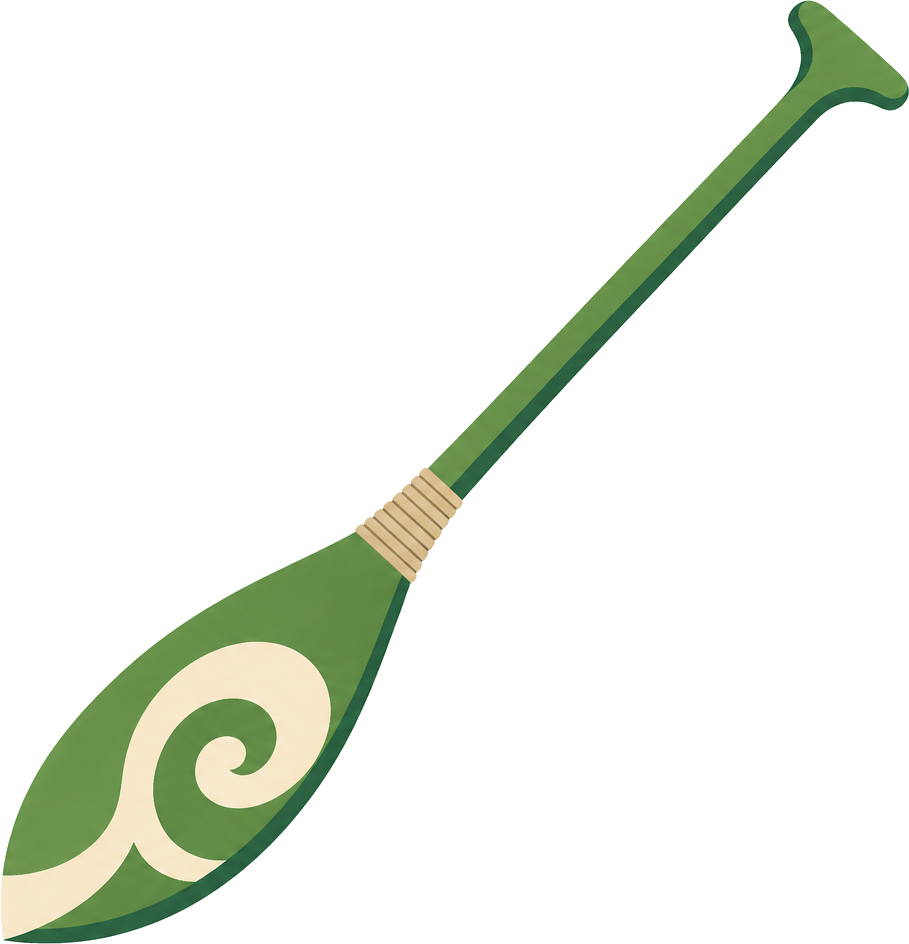
\includegraphics[height=1.05em]{img/hoe.png}}}
\newcommand{\ScaffoldIcons}[1]{\ifcase#1\or \HoeIcon\or \HoeIcon\hspace{0.22em}\HoeIcon\or \HoeIcon\hspace{0.22em}\HoeIcon\hspace{0.22em}\HoeIcon\fi}
\newcommand{\WorksheetTitle}[2]{
  \colorbox{mmtanSoft}{\parbox[c][2.0em][c]{0.975\linewidth}{\hspace{0.25em}{\Large\bfseries\textcolor{mmgreenDeep}{#1}\hfill\ScaffoldIcons{#2}}}}
  \par\vspace{0.08em}{\color{mmgreenLeaf}\rule{\linewidth}{2.0pt}}\par\vspace{0.04em}}
\newcommand{\MMAnswer}[2]{\begin{MMProblemCard}\raggedright\small\textbf{#1.} \textcolor{mmanswerColor}{\textbf{#2}}\par\end{MMProblemCard}}

\setbeamertemplate{background}{\begin{tikzpicture}[remember picture,overlay]\draw[black,line width=1.5pt,rounded corners=10pt]([xshift=0.45cm,yshift=-0.45cm]current page.north west) rectangle ([xshift=-0.45cm,yshift=0.45cm]current page.south east);\end{tikzpicture}}

\begin{document}
\begin{frame}[t]
\WorksheetTitle{Push Tasks - Answers}{3}
\vspace{-0.18em}
\begin{columns}[T,onlytextwidth]
\begin{column}{0.32\textwidth}\MMAnswer{1}{No — Sarah read the outer scale. 120° is correct; it is obtuse, not acute like a 60° angle.}\end{column}
\begin{column}{0.32\textwidth}\MMAnswer{2}{Tom read the outer scale instead of inner (130° on outer = 50° on inner), or misaligned the vertex.}\end{column}
\begin{column}{0.32\textwidth}\MMAnswer{3}{35° is acute (less than 90°). Correct measurement.}\end{column}
\end{columns}
\vspace{0.45em}
\begin{columns}[T,onlytextwidth]
\begin{column}{0.32\textwidth}\MMAnswer{4}{1. Place centre on vertex B. 2. Align 0° with ray BA. 3. Read where ray BC crosses the scale.}\end{column}
\begin{column}{0.32\textwidth}\MMAnswer{5}{1. Draw a baseline ray. 2. Place protractor centre at endpoint, 0° on ray. 3. Mark at 75°, then draw the second ray through the mark.}\end{column}
\begin{column}{0.32\textwidth}\MMAnswer{6}{No — 142° is obtuse (between 90° and 180°), not acute. The student confused the terms.}\end{column}
\end{columns}
\vspace{0.45em}
\begin{columns}[T,onlytextwidth]
\begin{column}{0.32\textwidth}\MMAnswer{7}{$\angle AOC = 30° + 50° = 80°$}\end{column}
\begin{column}{0.32\textwidth}\MMAnswer{8}{Reflex = 250°, so acute/obtuse = 360° - 250° = 110° (obtuse)}\end{column}
\begin{column}{0.32\textwidth}\MMAnswer{9}{$\angle COA = 360° - 85° - 95° = 180°$ (straight angle)}\end{column}
\end{columns}
\end{frame}
\begin{frame}[t]
\WorksheetTitle{Push Tasks - Answers}{3}
\vspace{-0.18em}
\begin{columns}[T,onlytextwidth]
\begin{column}{0.32\textwidth}\MMAnswer{10}{Estimate: approx 70--75°. To measure: place protractor centre at vertex, align baseline, read the scale.}\end{column}
\begin{column}{0.32\textwidth}\MMAnswer{11}{Roof angle = 22° from horizontal}\end{column}
\begin{column}{0.32\textwidth}\MMAnswer{12}{Off by 3°. Not within 1° tolerance — walls are out of square.}\end{column}
\end{columns}
\vspace{0.45em}
\begin{columns}[T,onlytextwidth]
\begin{column}{0.32\textwidth}\MMAnswer{13}{The centre was not on the vertex. Fix: ensure the protractor hole is exactly on the vertex point.}\end{column}
\begin{column}{0.32\textwidth}\MMAnswer{14}{1. Different scale reading (inner vs outer). 2. Different alignment of protractor centre or baseline.}\end{column}
\begin{column}{0.32\textwidth}\MMAnswer{15}{Acute = less than 90°. Sum of two acute angles < 180°, so $\angle AOC$ < 180° — not reflex. Could be acute (< 90°) or obtuse (90-180°).}\end{column}
\end{columns}
\vspace{0.45em}
\begin{columns}[T,onlytextwidth]
\begin{column}{0.32\textwidth}\MMAnswer{16}{360° ÷ 12 × 2 = 60°. Place protractor on the clock face centre, align 0° on 12, read at 2.}\end{column}
\begin{column}{0.32\textwidth}\MMAnswer{17}{360° ÷ 8 = 45°. Place protractor centre at pizza centre, align one cut line, read 45° to the next.}\end{column}
\begin{column}{0.32\textwidth}\MMAnswer{18}{3 hours × 30°/hour = 90°. A protractor can measure the angle directly from centre of clock if drawn.}\end{column}
\end{columns}
\end{frame}
\begin{frame}[t]
\WorksheetTitle{Push Tasks - Answers}{3}
\vspace{-0.18em}
\begin{columns}[T,onlytextwidth]
\begin{column}{0.32\textwidth}\MMAnswer{19}{180° - 67° = 113°. Inner and outer scales sum to 180°.}\end{column}
\begin{column}{0.32\textwidth}\MMAnswer{20}{Draw a 180° straight line, then measure 35° on the other side (180° + 35° = 215°). Or measure 145° the other way.}\end{column}
\begin{column}{0.32\textwidth}\MMAnswer{21}{47° + 62° + third = 180°, so third = 71°. The student was correct.}\end{column}
\end{columns}
\vspace{0.45em}
\begin{columns}[T,onlytextwidth]
\begin{column}{0.32\textwidth}\MMAnswer{22}{36° + 72° + 54° = 162°}\end{column}
\begin{column}{0.32\textwidth}\MMAnswer{23}{$\angle BOC = 155° - 60° = 95°$}\end{column}
\begin{column}{0.32\textwidth}\MMAnswer{24}{1. Centre on vertex. 2. Align baseline with 0°. 3. Read correct scale at the other ray.}\end{column}
\end{columns}
\vspace{0.45em}
\begin{columns}[T,onlytextwidth]
\begin{column}{0.32\textwidth}\MMAnswer{25}{Print scaling changes the actual size. Instead, read the measure given or use angle facts to calculate.}\end{column}
\begin{column}{0.32\textwidth}\MMAnswer{26}{Hour hand: at 3 = 90°, at 3:40 = 90° + (40/60×30°) = 110°. Minute hand: at 40 = 240°. Difference = |240° - 110°| = 130° (or 230° reflex). Smaller angle = 130°.}\end{column}
\begin{column}{0.32\textwidth}\MMAnswer{27}{Answers will vary. Example: $\angle AOB = 30°$, $\angle BOC = 50°$. Find $\angle AOC$. Answer: 80°.}\end{column}
\end{columns}
\end{frame}
\end{document}
